\documentclass[../main.tex]{subfiles}

\begin{document}

\section{Results}

As we saw in the code runner \textit{Code \ref{code:runner}}, we are executing with the combinations of the following parameters:

\begin{itemize}
    \item Block Dimension (Thread X and Y, respectively): [(4, 256), (8, 126), (16, 64), (32, 32), (64, 16), (128, 8), (256, 4)]
    \item Steps count: [100, 1000, 10000, 100000]
    \item Sizes: [100, 1000, 2000]
\end{itemize}

We decided to use a non square block size (except for \textit{32x32}) to try it out since in the previous parallel implementations we always tried dividing the grid into squares. Also, since we had a maximum of 1024 threads per block, if we multiply X and Y values it always satisfies that limit.

Before commenting on the comparison of the serial and CUDA execution times, comment that the serial executions were done in the moore cluster for the first assignment, so they are not done in the machine and is not fair, but we will focus in the time growth.

\subsection{Speedup}

We will do a comparison of the raw execution times between the parallel implementation and the serial counterparts in \textit{Figure \ref{fig:serial-vs-cuda}}, where we can see the execution times of the serial program compared to the mean execution time of CUDA in a logarithmic axis. We conclude that the CUDA program, even though slower in small grid sizes, scales better. In fact, we observe that the CUDA execution times do not change that much for any grid size, we can see it better in \textit{Table \ref{tab:cuda-times}}, where for the same Steps number, with different sizes, the serial time grows exponentially but the CUDA one stays the same, as with every matrix size and steps.

\begin{table}[!ht]
    \centering
\begin{tabular}{|c|c|c|c|}
\hline
Size & Steps  & CUDA Time    & Serial Time \\ \hline
100  & 100    & 0.450   & 0.010       \\
100  & 1000   & 4.562   & 0.110       \\
100  & 10000  & 44.394  & 1.020       \\
100  & 100000 & 445.999 & 10.180      \\ \hline
1000 & 100    & 0.482   & 1.340       \\
1000 & 1000   & 4.780   & 12.370      \\
1000 & 10000  & 47.734  & 109.600     \\
1000 & 100000 & 476.455 & 1072.980    \\ \hline
2000 & 100    & 0.532   & 5.330       \\
2000 & 1000   & 5.273   & 48.660      \\
2000 & 10000  & 52.656  & 476.730     \\
2000 & 100000 & 526.888 & 4310.410    \\ \hline
\end{tabular}
\caption{CUDA mean execution times}
\label{tab:cuda-times}
\end{table}

\begin{figure}[!ht]
    \centering
    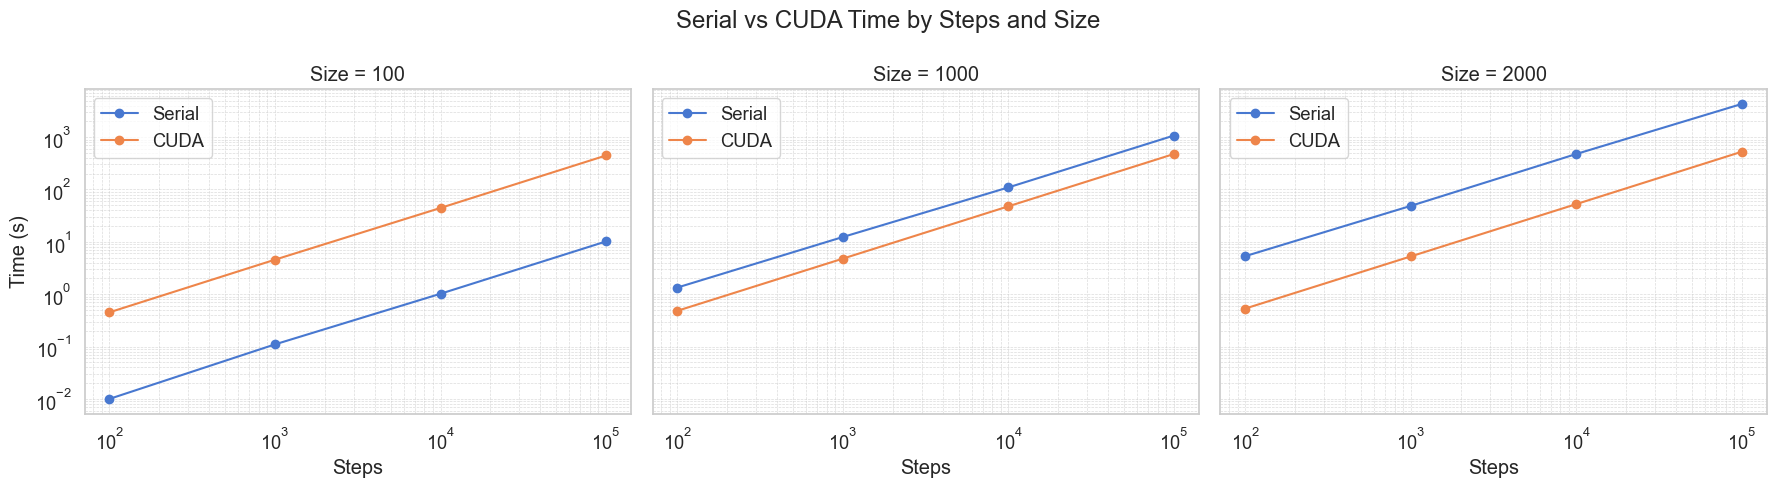
\includegraphics[width=0.9\linewidth]{media/images/serial-vs-cuda.png}
    \caption{Serial and CUDA comparison of raw times of execution}
    \label{fig:serial-vs-cuda}
\end{figure}

With these times extracted, we can calculate the speedups of \textit{Figure \ref{fig:speedup}} and \textit{Table \ref{tab:speedup}} with \textit{Formula \ref{eq:speedup}}, ending up having great speedups and with a clear improving tendency, with more speedup with fewer steps to make, which is logical with our implementation, since every step we have to launch two kernels in the GPU and synchronize them. 

\begin{equation}
    \begin{split}
        Speedup&=\frac{T_{Serial}}{T_{CUDA}}
    \end{split}
    \label{eq:speedup}
\end{equation}

\begin{figure}[!ht]
    \centering
    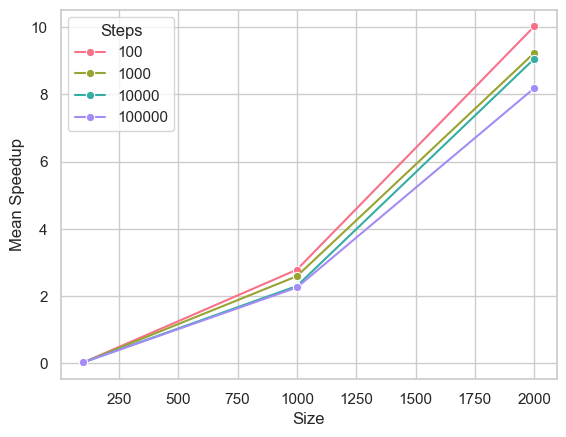
\includegraphics[width=0.7\linewidth]{media/images/speedup.png}
    \caption{CUDA implementation speedup}
    \label{fig:speedup}
\end{figure}

\begin{table}[!ht]
\centering
\begin{tabular}{|c|c|c|}
\hline
Size & Steps  & Speedup \\ \hline
\textbf{100}  & \textbf{100}    & \textbf{0.022}   \\
100  & 1000   & 0.024   \\
100  & 10000  & 0.023   \\
100  & 100000 & 0.023   \\ \hline
1000 & 100    & 2.782   \\
1000 & 1000   & 2.588   \\
1000 & 10000  & 2.296   \\
1000 & 100000 & 2.252   \\ \hline
2000 & 100    & 10.018  \\
2000 & 1000   & 9.228   \\
2000 & 10000  & 9.054   \\
\textbf{2000} & \textbf{100000} & \textbf{8.181}   \\ \hline
\end{tabular}
\caption{CUDA implementation speedup table}
\label{tab:speedup}
\end{table}

\subsection{Efficiency}

Now that we have speedups, we can calculate efficiency. 
We could divide our throughput by the installed GPU peak theoretical thoughput, but since we are more interested in the scalability of the Heat Diffusion problem, we will calculate the \textit{Relative Efficiency} defined as in \textit{Formula \ref{eq:relative-efficiency}}. 
This metric lets us know about how well does our program scale with larger problem sizes, to calculate it, we will compare the speedup with the largest and smallest executed problem size, bold rows in \textit{Table \ref{tab:speedup}}, which is \textbf{368.46}, meaning that the largest of the problem sizes that we tested, shows around \textit{400\%} more improvement than the smallest.

\begin{equation}
    \begin{split}
        Relative\_Efficiency&=\frac{Speedup_{\ Large\_Problem}}{Speedup_{\ Small\_Problem}}
    \end{split}
    \label{eq:relative-efficiency}
\end{equation}


\subsection{Block size comparison}

Lastly, as we executed the program with different block sizes, we will do a comparison of the different most expensive runs (\textit{100000 steps}) as we see in \textit{Figure \ref{fig:block-size}}, there we see that from those executions, the best ones are those with `taller' dimensions, meaning that the best were those that had a smaller X and bigger Y value. This behavior may be because if we look at \textit{heat\_kernel} function, we see that for every pixel we access its vertical and horizontal neighbors, and with this grid dimensions this memory may be already cached, otherwise it does not make much sense.

\begin{figure}[!ht]
    \centering
    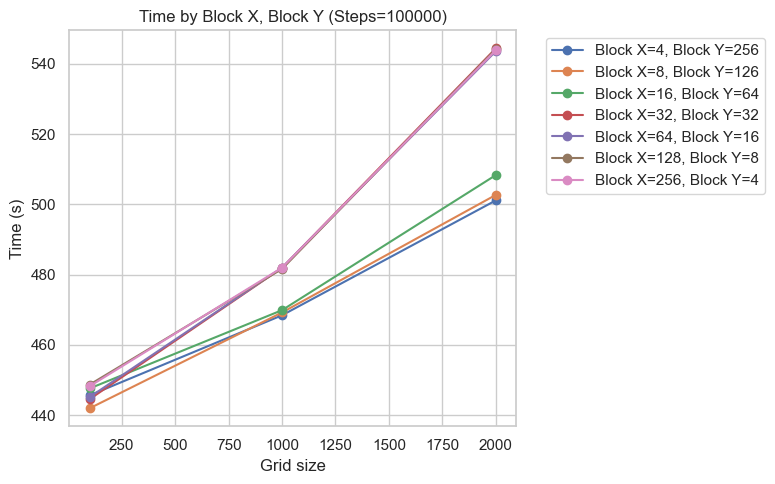
\includegraphics[width=0.9\linewidth]{media/images/time-by-block-dimensions.png}
    \caption{Comparison of time by different block dimension}
    \label{fig:block-size}
\end{figure}

\end{document}